\documentclass[border=6pt]{standalone}
\usepackage{tikz}
\usepackage[edges]{forest}
\usetikzlibrary{arrows.meta,positioning,calc,decorations.pathreplacing,shapes.geometric}
\begin{document}
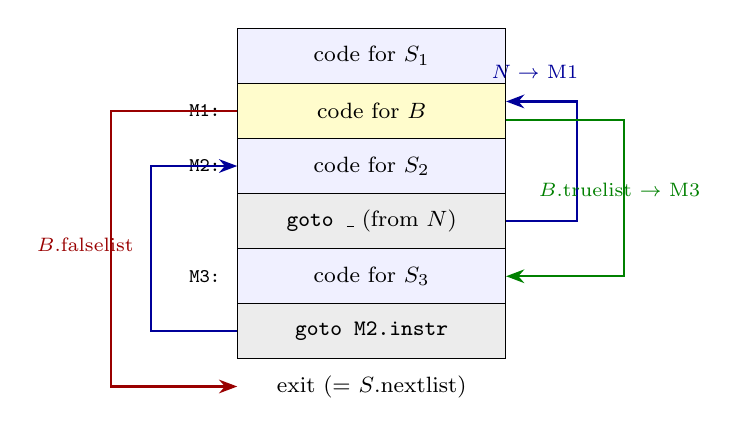
\begin{tikzpicture}[>=Stealth,font=\small,
 cell/.style={draw,minimum width=3.4cm,minimum height=0.7cm,align=center,font=\footnotesize},
 lab/.style={font=\scriptsize\ttfamily,anchor=east}]
\node[cell,fill=blue!6] (s1) at (0,0) {code for $S_1$};
\node[cell,fill=yellow!20] (b) at (0,-0.7) {code for $B$};
\node[cell,fill=blue!6] (s2) at (0,-1.4) {code for $S_2$};
\node[cell,fill=gray!15] (n) at (0,-2.1) {\texttt{goto \_} (from $N$)};
\node[cell,fill=blue!6] (s3) at (0,-2.8) {code for $S_3$};
\node[cell,fill=gray!15] (g) at (0,-3.5) {\texttt{goto M2.instr}};
\node[cell,draw=none] (ex) at (0,-4.2) {exit (= $S$.nextlist)};
\node[lab] at (-1.8,-0.7) {M1:}; \node[lab] at (-1.8,-1.4) {M2:}; \node[lab] at (-1.8,-2.8) {M3:};
\draw[->,thick,blue!60!black] (n.east) -- ++(0.9,0) |- ([yshift=0.12cm]b.east);
\draw[->,thick,green!50!black] ([yshift=-0.12cm]b.east) -- ++(1.5,0) |- (s3.east);
\draw[->,thick,red!60!black] (b.west) -- ++(-1.6,0) |- ([yshift=-0.0cm]ex.west);
\draw[->,thick,blue!60!black] (g.west) -- ++(-1.1,0) |- (s2.west);
\node[font=\scriptsize,anchor=west,green!50!black] at (2.0,-1.7) {$B$.truelist $\to$ M3};
\node[font=\scriptsize,anchor=west,blue!60!black] at (1.4,-0.2) {$N \to$ M1};
\node[font=\scriptsize,anchor=east,red!60!black] at (-2.9,-2.4) {$B$.falselist};
\end{tikzpicture}
\end{document}
